\begin{lemma}
    \label{conics/30/lemma}
    The distance of a point $\vec{P}$ from a line $L: \vec{n}^T\vec{x}=c$ is given by:
    \begin{align}
    d = \frac{\abs{c-\vec{P}^T\vec{n}}}{\norm{\vec{n}}}   
    \end{align}
    \end{lemma}
    
\begin{definition}
\label{conics/30/def}
The locus of $\vec{P}$ such that 
\begin{align}
\frac{\norm{\vec{P}-\vec{F}}}{d} = e    
\end{align}
is known as a conic section. The line $L$ is known as the directrix and the point $\vec{F}$ is the focus. $e$ is defined to be 
the eccentricity of the conic.  
\begin{enumerate}
    \item For $e = 1$, the conic is a parabola
    \item For $e < 1$, the conic is an ellipse
    \item For $e > 1$, the conic is a hyperbola
\end{enumerate}
\end{definition}

\begin{theorem}
The equation of  a conic is given by any conicis given by:
\begin{align}
\vec{x}^T(t\vec{I}-\vec{n}\vec{n}^T)\vec{x}+2(c\vec{n}-t\vec{F})^T\vec{x}+t\norm{\vec{F}}^2-c^2&=0
\end{align}
%
where
\begin{align}
    t=\frac{\norm{\vec{n}}^2}{e^2}
\end{align}
\end{theorem}

\begin{proof}

Using Definition \ref{conics/30/def} and Lemma \ref{conics/30/lemma},  for any point $\vec{x}$ on the conic,
\begin{align}
\norm{\vec{x}-\vec{F}}^2=e^2 \frac{({c-\vec{x}^T\vec{n}})^2}{\norm{\vec{n}}^2}\label{conics/30/eq:1} \\
t(\vec{x}-\vec{F})^T(\vec{x}-\vec{F})=(c-\vec{x}^T\vec{n})^2
\\
t(\vec{x}^T\vec{x}-2\vec{F}^T\vec{x}+\norm{\vec{F}}^2)=c^2+(\vec{x}^T\vec{n})^2-2c\vec{x}^T\vec{n}\\
t\vec{x}^T\vec{x}-(\vec{x}^T\vec{n})^2-2t\vec{F}^T\vec{x}+2c\vec{n}^T\vec{x}=c^2-t\norm{\vec{F}}^2\\
t\vec{x}^T\vec{I}\vec{x}-\vec{x}^T\vec{n}\vec{n}^T\vec{x}+2(c\vec{n}-t\vec{F})^T\vec{x}=c^2-t\norm{\vec{F}}^2\\
\vec{x}^T(t\vec{I}-\vec{n}\vec{n}^T)\vec{x}+2(c\vec{n}-t\vec{F})^T\vec{x}+t\norm{\vec{F}}^2-c^2=0
\end{align}
\end{proof}
% \begin{corollary}
% The equation for parabola assuming $\lambda=\norm{\vec{n}}^2$ will be: 
% \begin{align}
% \vec{x}^T(\lambda\vec{I}-\vec{n}\vec{n}^T)\vec{x}+2(c\vec{n}-\lambda\vec{F})^T\vec{x}+\lambda\norm{\vec{F}}^2-c^2&=0\label{conics/30/eq:8}
% \end{align}
% \end{corollary}
From the given information,
\begin{align}
\vec{F}=\myvec{2\\0},
\vec{n}=\myvec{1\\0},
c=-2\label{conics/30/eq:9},
t=1
\end{align}
Hence, substituting from \eqref{conics/30/eq:9}, the equation of the conic is 
\begin{align}
\vec{x}^T\myvec{0&0\\0&1}\vec{x}+2\myvec{-4&0}\vec{x}+0&=0\label{conics/30/eq:11}
\end{align}
%
Replacing $\vec{x}$ by $\myvec{x\\y}$ in \eqref{conics/30/eq:11} gives
\begin{align}
y^2=8x
\end{align}
which is plotted in Fig.  \ref{conics/30/fig:parabola}.	
\begin{figure}[!ht]
    \centering
    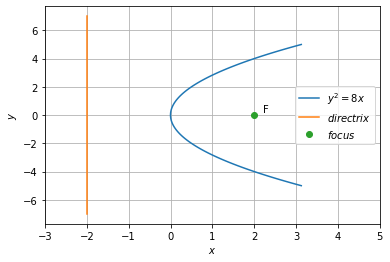
\includegraphics[width=\columnwidth]{solutions/su2021/2/30/figure4.png}
    \caption{Parabola $y^2=8x$ }
    \label{conics/30/fig:parabola}	
    \end{figure}
    
